\chapter{Il Livello di Trasporto}
\thispagestyle{chapterInit}
\paragraph{Obbiettivi}
    \begin{itemize}
        \item Capire i principi che sono alla base dei servizi di livello di trasporto:
            \subitem \textit{Multiplexing/de-multiplexing}
            \subitem Trasferimento dati affidabile
            \subitem Controllo di flusso
            \subitem Controllo di congestione
        \item Descrivere i protocolli del livello di trasporto di Internet:
            \subitem \Acrshort*{TCP}: Trasposto orientato alla connessione
            \subitem Controllo di congestione TCP
            \subitem \Acrshort*{UDP}: Trasporto non orientato alla connessione
    \end{itemize}
\section{Servizi a livello di trasporto}
    \paragraph{Introduzione} I \textbf{protocolli di trasporto} forniscono la comunicazione logica tra processi applicativi di host diversi. I protocolli di trasporto vengono eseguiti negli host "terminali" ovvero quelli che generano o consumano i dati. Dal lato di inviante il protocollo di trasporto divide in diversi segmenti i dati ricevuti dal livello di applicazione e li invia al livello di rete. Dal lato di ricevente il protocollo di trasporto riassembla i segmenti ricevuti e li invia al livello di applicazione.
    \paragraph{\Acrshort*{TCP}} Il \acrfull*{TCP} è un protocollo di trasporto orientato alla connessione. Il \Acrshort*{TCP} fornisce un trasferimento affidabile dei dati, controllo di flusso e controllo di congestione.
    \paragraph{\Acrshort*{UDP}} L'\acrfull*{UDP} è un protocollo di trasporto non orientato alla connessione. L'\Acrshort*{UDP} non fornisce trasferimento affidabile dei dati, controllo di flusso e controllo di congestione.
    \paragraph{Servizi non disponibili} Al momento in internet non è disponibile un servizio di garanzia su ritardi (latenza), e non è disponibile un servizio di garanzia sulla banda (velocità di trasferimento).
\section{\textit{Multiplexing e De-multiplexing}}
    \paragraph{Introduzione} Il \textit{\textbf{multiplexing}} è il processo di invio di dati da più \textit{socket} a un'unica connessione, per identificare il \textit{socket} di destinazione si utilizza un \textit{\textbf{port number}}. Il \textit{\textbf{de-multiplexing}} è il processo di invio dei dati ricevuti al socket corretto in base al port number.
    \subsection{\textit{De-multiplexing}}
        \paragraph{Come funziona} In primo luogo quando l'\textit{host} riceve un segmento \Acrshort*{IP} contenente: \Acrshort*{IP} del mittente, \Acrshort*{IP} del destinatario, protocollo di trasporto, porta di destinazione e porta di sorgente. L'\textit{host} utilizza l'indirizzo \Acrshort*{IP} del destinatario e la porta di destinazione per inviare il segmento al processo corretto.
        \subsubsection{\textit{De-multiplexing} senza connessione}
            Per eseguire il de-multiplexing senza connessione si crea un \textit{socket} per ricevere i dati. Il \textit{socket} è ora associato a una porta ed a un indirizzo \Acrshort*{IP}. Quando l'\textit{host} riceve il segmento \Acrshort*{UDP}, viene controllato che il numero di porta di destinazione sia uguale alla porta del \textit{socket}. Se il numero di porta non corrisponde il segmento viene scartato. Se invece il numero di porta corrisponde il segmento viene inviato al processo associato al \textit{socket}.
            \begin{figure}[H]
                \centering
                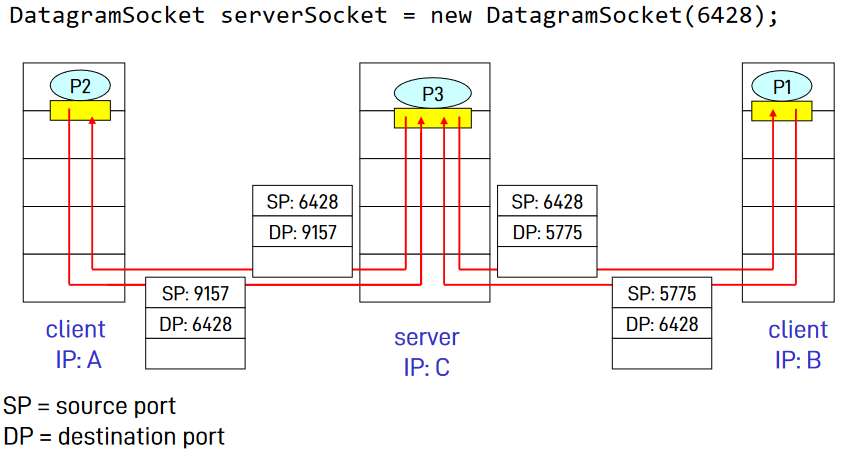
\includegraphics[width=0.5\textwidth]{03/DemultiplexingSenzaConnessione.png}
                \caption{\textit{De-multiplexing} senza connessione}
            \end{figure}
        \subsubsection{\textit{De-multiplexing} orientato alla connessione}
            Quando si utilizza un protocollo orientato alla connessione (\Acrshort*{TCP}), il processo di \textit{de-multiplexing} è leggermente diverso. Il \textit{socket} infatti è costituito da quattro parametri: indirizzo \Acrshort*{IP} del mittente, indirizzo \Acrshort*{IP} del destinatario, numero di porta di sorgente e numero di porta di destinazione. Quando l'\textit{host} riceve un segmento \Acrshort*{TCP} controlla che i quattro parametri del \textit{socket} corrispondano ai quattro parametri del segmento. Se i parametri non corrispondono il segmento viene scartato, altrimenti viene inviato al processo associato al \textit{socket}. Un \textit{host} può supportare più \textit{socket} contemporaneamente purché cambi almeno uno dei quattro parametri, inoltre i \textit{web server} sono un chiaro esempio di applicazione che utilizza più \textit{socket} contemporaneamente (su \texttt{HTTP/1.0} un \textit{socket} per ogni richiesta).\footnote{Se viene allocata una porta ad una connessione, la porta non può essere utilizzata da altre connessioni, quindi nel caso di un \textit{web server} è vero che questo ascolta sulla porta \texttt{80}, ma quando un client si connette al server, il server apre un \textit{socket} con una porta dinamica.}
            \begin{figure}[H]
                \centering
                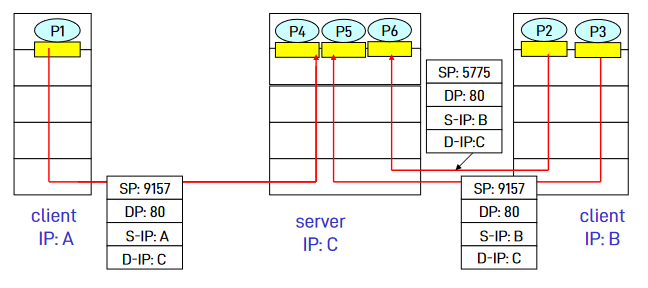
\includegraphics[width=0.5\textwidth]{03/DemultiplexingConConnessione.png}
                \caption{De-multiplexing orientato alla connessione}
            \end{figure}
    \subsection[Porte \texttt*{TCP}-\texttt{UDP}]{Porte \Acrshort*{TCP}-\Acrshort*{UDP}}
        La destinazione finale di un segmento non è un host ma un processo. L'interfaccia tra l'applicazione e il livello di trasporto è chiamata \textbf{socket} o \textbf{porta} (nel caso di \Acrshort*{UDP} e \Acrshort*{TCP}). Un \textbf{socket} è un indirizzo \Acrshort*{IP} e un numero di porta. Un \textit{\textbf{port number}} è un numero a $16$ bit che identifica un processo all'interno di un host. Esiste una mappatura biunivoca tra un \textit{\textbf{port number}} e un processo. I servizi standard utilizzano porte ben note con valori tra $0$ e $1023$. I processi non-standard e le connessioni in ingresso a un client usano numeri fino a $25535$ ($16$ bit).
        \paragraph{Numeri di porte}
            I numeri di porta si classificano come segue:
            \begin{description}
                \item[Statici] Per i servizi standard, es. \Acrshort*{HTTP} (\texttt{80}), \Acrshort*{FTP} (\texttt{21}), \Acrshort*{SSH} (\texttt{22}), \texttt{Telnet} (\texttt{23}), \Acrshort*{SMTP} (\texttt{25}), \Acrshort*{POP3} (\texttt{110}), \Acrshort*{IMAP} (\texttt{143}), \Acrshort*{HTTPS} (\texttt{443}), ecc.
                \item[Dinamici] (o ``ephemeral'') per le connessioni in uscita o per porte allocate dinamicamente, es. client web, client \Acrshort*{FTP}, client \Acrshort*{SSH}, client \texttt{Telnet}, client \Acrshort*{SMTP}, client \Acrshort*{POP3}, client \Acrshort*{IMAP}, client \Acrshort*{HTTPS}, ecc.
            \end{description}
            Inoltre è importante dire che le porte di sorgente e di destinazione non sono le stesse in quanto la porta di sorgente è una porta dinamica assegnata dal sistema operativo.
\section[Trasporto senza connessione: \texttt{UDP}]{Trasporto senza connessione: \Acrshort*{UDP}}
    \paragraph{Caratteristiche} L'\acrfull*{UDP} è un protocollo di trasporto senza connessione, offre un servizio \textit{best effort} e non fornisce garanzie di consegna, ordine o duplicazione dei dati. Questo in quanto non ha \textit{handshake} iniziale e non mantiene alcuno stato di connessione. 
    \paragraph{Perché esiste \Acrshort*{UDP}} Non richiede di stabilire una connessione, è semplice e veloce, Header di segmento corti, senza controllo di congestione.
    \subsection{Header}
        \begin{figure}[H]
            \centering
            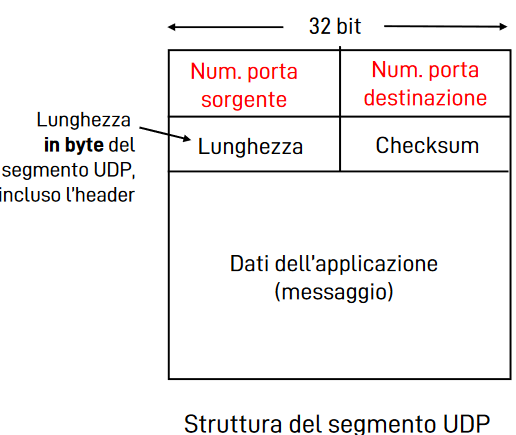
\includegraphics[width=0.3\textwidth]{03/UDPHeader.png}
            \caption{Header di un segmento \Acrshort*{UDP}}
        \end{figure}
        \begin{description}
            \item[Porta di sorgente] Numero di porta del processo mittente.
            \item[Porta di destinazione] Numero di porta del processo destinatario.
            \item[Lunghezza] Lunghezza del segmento in byte.
            \item[\textit{Checksum}] Utilizzato per rilevare errori nel segmento.
        \end{description}
        \subsubsection{\textit{Checksum}}
            Il \textit{checksum} è un campo a 16 bit che viene utilizzato per rilevare errori nel segmento. Questo viene calcolato da entrambe le parti: viene trattato il contenuto come una sequenza di $ 16 $ bit e si sommano tutti i bit (se presente riporto questo viene sommato a sua volta) e viene eseguito il complemento a 1. Il mittente invia il \textit{checksum} calcolato nel segmento e il ricevente calcola il \textit{checksum} del segmento ricevuto e lo confronta con il \textit{checksum} ricevuto. Se i due \textit{checksum} non corrispondono il segmento viene scartato.
\section[Trasferimento dati affidabile]{Principi del trasferimento dati affidabile}
    \subsection[Automatic Repeat reQuest (\texttt{ARQ})]{\acrfull*{ARQ}}
        \acrfull*{ARQ} è una classe di protocolli che ``cercano'' di recuperare i segmenti persi o danneggiati. Questa classe usa dei pacchetti speciali per notificare al mittente che un segmento è stato perso o danneggiato. Questi pacchetti speciali sono chiamati \acrfull*{ACK} e \acrfull*{NACK}.
        \paragraph{Esempi di protocolli basati su \Acrshort*{ARQ}} \begin{itemize}
            \item \textit{Stop-and-Wait}
            \item \textit{Go-Back-N}
            \item \textit{Selective Repeat}
            \item \Acrshort*{TCP}
            \item il protocollo \Acrshort*{MAC} (al livello 2) dei sistemi \Acrshort*{Wi-Fi}
        \end{itemize}
    \subsection{\textit{Stop-and-Wait}}
        Nel protocollo \textit{Stop-and-Wait} il mittente invia una \Acrshort*{PDU} e ne mantiene una copia in memoria, imposta dunque un \textit{timeout} su quel \Acrshort*{PDU}. Attende poi un \Acrshort*{ACK} dal ricevente, se non riceve l'\Acrshort*{ACK} entro il \textit{timeout} invia nuovamente la \texttt{PDU}. Se invece riceve l'\Acrshort*{ACK} controlla che questo non contenga errori, che sia il numero di sequenza corretto e che sia per la \Acrshort*{PDU} inviata. Se tutto è corretto invia la prossima \Acrshort*{PDU}. Il ricevente quando riceve una \Acrshort*{PDU} controlla che il numero di sequenza sia corretto e che la \Acrshort*{PDU} non abbia errori, se tutto è corretto invia un \Acrshort*{ACK} al mittente, de-capsula la \Acrshort*{PDU} ai livelli superiori. Se sono presenti errori nella \Acrshort*{PDU} il ricevente esegue il \textit{drop} della \Acrshort*{PDU}.
        \subsubsection{Efficienza dello \textit{Stop-and-Wait}}
            Assumendo una banda $ R = 1 G-bit/s, 15ms $ di ritardo di propagazione, lunghezza del messaggio $ L = 8000bit $, allora il tempo di trasmissione sarà: $T_{trans} = \frac{L}{R} = \frac{80000}{10^9} = 8\mu s$. Mentre il \textit{throughput} percepito a livello applicativo sarà: $ \frac{L}{T_{trans}+RTT}= \frac{8000}{8\mu s + 30ms} = 33 Kbps $.\footnote{Aggiungiamo della formula il \Acrshort*{RTT} ovvero il \acrlong*{RTT} che è il tempo che impiega un pacchetto per andare dal mittente al ricevente e ritornare indietro, nel nostro caso lo aggiungiamo per il pacchetto di \Acrshort*{ACK} ed è di $ 30ms $.} Dunque anche se la nostra banda è di $ 1 Gbps $ il \textit{throughput} percepito a livello applicativo è di $ 33 Kbps $, l'efficienza dunque è: $ \frac{T_{trans}}{T_{trans}+RTT} = \frac{0.008}{0.008+30} = 0.00027 $ ovvero $ 0.027\% $.
    \subsection{Protocolli con \textit{pipelining}}
        I protocolli con \textit{pipelining} permettono di inviare più segmenti successivi senza attendere l'\Acrshort*{ACK} del segmento precedente, si allarga dunque il range dei pacchetti di sequenza accettabili. Questo permette di aumentare l'efficienza del trasferimento dati. Esempio di protocolli con \textit{pipelining} sono \textit{Go-Back-N} e \textit{Selective Repeat}.
        \subsubsection{\textit{Throughput} in presenza di \textit{pipelining}}
            Assumiamo la stessa situazione precedente ed un \textit{pipelining} di $ N = 3 $ allora il \textit{throughput} sarà: $$ \frac{3L}{T_{trans}+RTT} = \frac{24000}{8\mu s + 30ms} = 100 Kbps $$questo è un miglioramento del $ 300\% $ rispetto allo \textit{Stop-and-Wait}. In generale il \textit{throughput} rispetto al \textit{pipelining} con $ N $ segmenti in parallelo è: $ \frac{N \cdot L}{RTT + T_{trans}} $. Il parametro $ N $ è detto \textit{window size} o "dimensione della finestra".
        \subsubsection{Definizioni}
            \begin{description}
                \item[\acrfull*{W_T}] Insieme di \Acrshort*{PDU} che il mittente può inviare senza attendere un \Acrshort*{ACK} del ricevente.
                    \subitem Grande al massimo come la memoria allocata dal sistema operativo.
                    \subitem \Acrshort*{W_T_d} indica la dimensione della finestra.
                \item[\acrfull*{W_R}] Insieme di \Acrshort*{PDU} che il ricevente può ricevere può accettare e memorizzare.
                    \subitem Grande al massimo come la memoria allocata dal sistema operativo.
                \item[\acrfull*{W_LOW}] Puntatore al primo segmento trasmesso ma non ancora confermato.
                \item[\acrfull*{W_HIGH}] Indica l'ultimo segmento già trasmesso della finestra di trasmissione \Acrshort*{W_T}.
            \end{description}
        
        \begin{figure}[H]
            \centering
            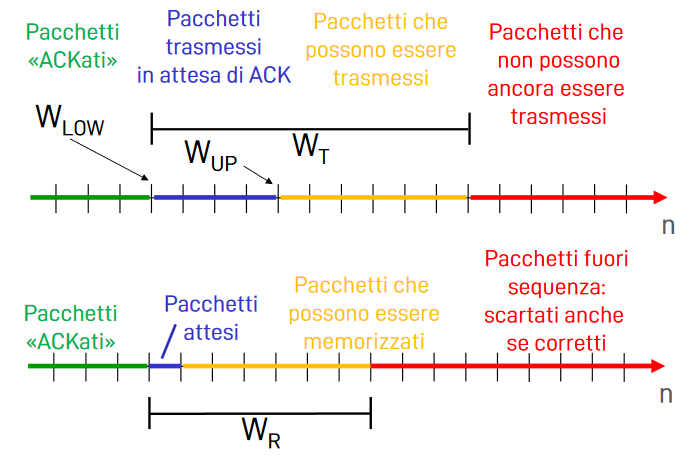
\includegraphics[width=0.5\textwidth]{03/finestrePipelining.png}
            \caption{Finestre di trasmissione e di ricezione}
        \end{figure}
        \subsubsection[ACKnowledgment (\Acrshort*{ACK})]{\acrfull*{ACK}}
            Esistono vari tipi di \Acrshort*{ACK} a seconda del protocollo utilizzato, abbiamo dunque:
            \begin{itemize}
                \item \Acrshort*{ACK} individuale il cui compito è quello di indicare la corretta ricezione di uno specifico pacchetto - \texttt{ACK($n$)} vuol dire ho ricevuto il pacchetto $n$.
                \item \Acrshort*{ACK} cumulativo il cui compito è quello di indicare la corretta ricezione di tutti i pacchetti fino a quello specificato - \texttt{ACK($n$)} vuol dire ho ricevuto tutti i pacchetti fino a $n$ (escluso), mi aspetto il pacchetto $n$.
                \item \Acrshort*{ACK} negativo o \Acrshort*{NACK} il cui compito è quello di indicare la mancata ricezione di un pacchetto - \texttt{NACK($n$)} vuol dire non ho ricevuto il pacchetto $n$, invialo nuovamente.
                \item Esiste poi la tecnica del ``\textbf{Piggybacking}", ovvero l'inserimento dell'\Acrshort*{ACK} (di un pacchetto precedente) all'interno di un pacchetto dati successivo.
            \end{itemize}
        \subsubsection{\textit{Go-Back-N}}
            Quando si sceglie di usare il protocollo del tipo \textit{Go-Back-N} questo consiste in: il mittente invia fino ad un numero $ n $ di pacchetti senza aver ricevuto prima \Acrshort*{ACK}, quando un pacchetto è stato ricevuto correttamente viene inviato un \Acrshort*{ACK} cumulativo, se un pacchetto non è stato ricevuto allora i pacchetti successivi vengono scartati in attesa del pacchetto mancante. Dopo un periodo di \textit{timeout} il mittente invia nuovamente tutti i pacchetti a partire dal pacchetto mancante, basandosi sull'ultimo \Acrshort*{ACK} ricevuto. La finestra di trasmissione \Acrshort*{W_T} è dunque composta da $ n $ pacchetti e non viene spostata finché non si riceve un \Acrshort*{ACK} cumulativo, mentre la finestra di ricezione \Acrshort*{W_T} è composta da un solo pacchetto.
        \subsubsection{\textit{Selective Repeat}}
            Nel paradigma del \textit{selective repeat} vengono usati \Acrshort*{ACK} singoli, inoltre è presente una finestra di ricezione \Acrshort*{W_R} composta da $ m $ pacchetti, ciò significa che anche se un pacchetto ricevuto fuori sequenza viene ricevuto allora questo viene comunque ``salvato" all'interno di un buffer in attesa del pacchetto nell'ordine corretto. Anche il mittente in caso di \Acrshort*{ACK} fuori sequenza conserva in memoria questo dato e non lo scarta. Quello che succede se un pacchetto non viene ricevuto ma qualche pacchetto (fino a $m-1$) successivo viene ricevuto correttamente è che il mittente invia nuovamente solo il pacchetto mancante, mentre i pacchetti successivi, se sono già stati \texttt{ACK'ati}, non vengono inviati nuovamente e la trasmissione riprende dal primo pacchetto non \texttt{ACK' ato}.
        \paragraph{Spazio dei numeri di sequenza}
            Solitamente se si hanno $ k $ bit a disposizione, per il dominio del numero di sequenza, allora si usa un periodo pari a $ 2^k $, ovvero il periodo massimo con quello spazio di bit. Le finestre di trasmissione per non avere conflitti devono avere somma inferiore al periodo, quindi \Acrshort*{W_T_d}$+$\Acrshort*{W_R_d}$< 2^k $.\footnote{I conflitti nel caso nel quale ``La somma delle finestre di trasmissione e di ricezione sia maggiore del periodo dei numeri di sequenza" sono dovuti al fatto che in questa situazione in caso di perdita di pacchetti di controllo (\Acrshort*{ACK}/\Acrshort*{NACK}) ma trasmissione corretta dei pacchetti dati, il mittente non saprebbe se il pacchetto è stato ricevuto correttamente o meno il che provoca un \textit{timeout} e la ritrasmissione dei pacchetti dati per persi, però dato che abbiamo già ricevuto i pacchetti dati abbiamo spostato la finestra di ricezione ed il ricevente potrebbe scambiare come per buoni la ritrasmissione dei pacchetti dati che il mittente ha dato per persi.} 
\section[Trasporto Orientato Connessione \texttt{TCP}]{Trasporto orientato alla connessione \Acrshort*{TCP}}
    \paragraph{\Acrshort*{TCP} - vari standard \Acrshort*{RFC}} Il \acrfull*{TCP} è un protocollo di trasporto orientato alla connessione, è stato standardizzato nel \texttt{\Acrshort*{RFC} 793} e successivamente aggiornato con il \texttt{\Acrshort*{RFC} 1122}, \texttt{\Acrshort*{RFC} 1323}, \texttt{2018}, \texttt{2581} ed è in continuo aggiornamento. Questo prevede una connessione \underline{punto-punto} tra mittente e destinatario, è presente un flusso di byte affidabile e consegnato in ordine senza limiti, è presente un meccanismo di \textit{pipelining} e di controllo di congestione per non sovraccaricare la rete. La connessione inoltre (anche se a livelli inferiori non lo è) è \textit{\underline{full-duplex}} ovvero entrambi i lati possono inviare e ricevere dati contemporaneamente. Inoltre il \Acrshort*{TCP} è un protocollo \textit{\underline{stateful}} ovvero mantiene uno stato della connessione, infatti si dice che è orientato alla connessione. Infine \Acrshort*{TCP} ha un ``flusso controllato'' ovvero il trasmettitore non può inviare dati se il ricevente non è pronto a riceverli.
    \subsection[Struttura di un pacchetto \texttt{TCP}]{Struttura di un pacchetto \Acrshort*{TCP}}
        \begin{figure}[H]
            \centering
            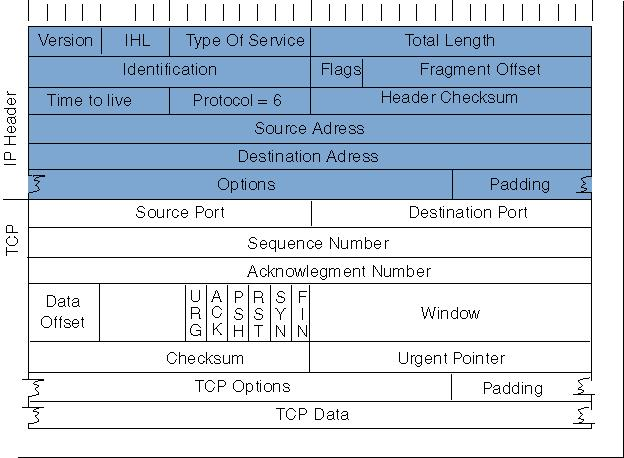
\includegraphics[width=0.45\textwidth]{03/pacchettoTCP.jpg}
            \caption{Struttura di un pacchetto \Acrshort*{TCP} } 
        \end{figure}
        {\footnotesize Immagine tratta da \href{https://commons.wikimedia.org/wiki/File:Ntwk_tcp_header.jpg}{Wikimedia Commons} di Gopalpaliwal at English Wikibooks il file è rilasciato sotto licenza Creative Commons \href{https://creativecommons.org/licenses/by-sa/3.0/deed.en}{Attribution-Share Alike 3.0 Unported}.}
        Nel pacchetto \Acrshort*{TCP} sono presenti i seguenti campi principali:
        \begin{description}
            \item[\textit{Source Port}] Porta di sorgente.
            \item[\textit{Destination Port}] Porta di destinazione.
            \item[\textit{Sequence Number}] Numero di sequenza del primo byte del segmento.
            \item[\Acrlong*{ACK} \textit{Number}] Numero di sequenza del prossimo byte atteso.
            \item[\textit{Data Offset}] Lunghezza dell'header in parole di 32 bit.
            \item[\Acrshort*{URG}] Flag che indica la presenza di dati urgenti.
            \item[\Acrshort*{ACK}] Flag che indica la presenza di un campo \Acrshort*{ACK}.
            \item[\Acrshort*{PSH}] Flag che indica che i dati devono essere passati al livello superiore.
            \item[\Acrshort*{PST}] Flag che indica l'inizio di una connessione.
            \item[\Acrshort*{SYN}] Flag che indica la sincronizzazione dei numeri di sequenza.
            \item[\Acrshort*{FIN}] Flag che indica la chiusura della connessione.
            \item[\textit{Window}] Dimensione della finestra di ricezione. (\Acrshort*{RWND})
            \item[\textit{checksum}] Utilizzato per rilevare errori nel segmento (contiene oltre agli header \Acrshort*{TCP} e i dati dei livelli superiori anche i campi \Acrshort*{IP} come l'indirizzo \Acrshort*{IP} del mittente e del destinatario, la lunghezza del segmento, il protocollo di trasporto, ecc.).
            \item[\textit{Urgent Pointer}] Puntatore ai dati urgenti.
            \item[\textit{\Acrshort*{TCP} Options}] Opzioni aggiuntive. (opzionali)
            \item[\textit{Padding}] Padding per allineare il segmento a 32 bit.
            \item[\textit{Data}] Dati del segmento.
        \end{description}
        \paragraph{\acrfull*{RWND}} La finestra di ricezione è un campo a $16$ bit che indica la dimensione della finestra di ricezione del ricevente. Questo campo è utilizzato per il controllo di flusso, infatti il mittente non può inviare dati se la finestra di ricezione del ricevente è piena. La finestra di ricezione è un campo a $16$ bit, quindi la dimensione massima della finestra di ricezione è di $ 2^{16} - 1 = 65535 $ byte. In base alla velocità della banda questo campo può essere modificato per evitare che il mittente non sfrutti tutta la banda disponibile.
        \paragraph{Numeri di sequenza \Acrshort*{ACK} di \Acrshort*{TCP}} I numeri di sequenza di \Acrshort*{TCP} sono a $32$ bit, questo significa che il numero di sequenza può variare tra $ 0 $ e $ 2^{32} - 1 = 4294967295 $. Il numero di sequenza nella direzione mittente-ricevente può essere diverso da quello nella direzione ricevente-mittente, questo perché i numeri di sequenza sono indipendenti nelle due direzioni, inoltre non è detto che i numeri di sequenza inizino da $ 0 $, infatti possono iniziano solitamente da un numero casuale. Durante la trasmissione di un pacchetto mittente-ricevente può essere allegato anche un campo \Acrshort*{ACK} per la conferma della ricezione del pacchetto precedente tra ricevente-mittente (stessa cosa per la direzione opposta).
        \subsubsection{Lunghezza massima segmento \Acrshort*{MSS} e \Acrshort*{MTU}}
            In quanto il \Acrshort*{TCP} lavora per byte cerca sempre di non inviare un singolo byte solo in quanto sarebbe uno spreco di risorse e di banda. Allo stesso tempo non si può inviare un segmento troppo grande in quanto potrebbe essere frammentato a livello di rete. Viene dunque introdotta una "lunghezza massima" detta \acrfull*{MSS} che indica la lunghezza massima di un segmento \Acrshort*{TCP}. La \Acrshort*{MSS} è calcolata come la \acrfull*{MTU} che è la lunghezza massima di un pacchetto che può essere inviato su una rete a livello di collegamento. A sua volta la \Acrshort*{MTU} viene calcolata da passati al livello \textit{data-link} e può variare da rete a rete. La \Acrshort*{MSS} si riferisce non alla lunghezza di tutto il segmento \Acrshort*{TCP} ma solo al \textit{payload}, ovvero il campo dati del segmento \Acrshort*{TCP}.
            \paragraph{Come si sceglie \Acrshort*{MSS}?} Non esistono meccanismi per comunicarlo, viene dunque adottato un modello del tipo \textit{trial\& error}, ovvero il mittente invia un segmento con una \Acrshort*{MSS} di dimensione $ X $ se si nota che i livelli inferiori sopportano la dimensione $ X $ allora si aumenta la dimensione della \Acrshort*{MSS}, altrimenti se si nota che qualche messaggio inizia ad essere perso si riduce la dimensione della \Acrshort*{MSS}.
                \subparagraph{Valodi di default}: \begin{itemize}
                    \item \Acrshort*{MTU} di ethernet: $ 1500 $ byte (payload inseribile al livello 2)
                    \item Header \Acrshort*{IP}: $ 20 $ byte
                    \item Header \Acrshort*{TCP}: $ 20 $ byte
                    \item \Acrshort*{MSS} di default: $ 1460 $ byte
                \end{itemize}
                \subparagraph{``\textit{Least maximum}"} La più piccola \Acrshort*{MTU} impostabile per \Acrshort*{IP} è di $ 576 $ byte, questo dunque la \Acrshort*{MSS} di minima impostabile è di $ 536 $ byte.
    \subsection[Setup della connessione \texttt{TCP} - \textit{handshake}]{Setup della connessione \Acrshort*{TCP} - \textit{handshake}}
        La procedura di apertura di una connessione \Acrshort*{TCP} è detta \textit{three-way handshake}, questa procedura è composta dai seguenti passaggi:
        \begin{enumerate}
            \item \textbf{Host A} invia un segmento \Acrshort*{TCP} con il flag \Acrshort*{SYN} impostato a \texttt{1} e la porta di sorgente $ A $ e la porta di destinazione $ B $.
            \item \textbf{Host B} riceve il segmento \Acrshort*{TCP} e invia un segmento \Acrshort*{TCP} con il flag \Acrshort*{SYN} impostato a \texttt{1} e il flag \Acrshort*{ACK} impostato a \texttt{1} (avvenuta la ricezione del segmento di \Acrshort*{SYN}) e la porta di sorgente $ B $ e la porta di destinazione $ A $.
            \item \textbf{Host A} riceve il segmento \Acrshort*{TCP} e invia un segmento \Acrshort*{TCP} con il flag \Acrshort*{ACK} impostato a \texttt{1} (avvenuta la ricezione del segmento di \Acrshort*{SYN}) e la porta di sorgente $ A $ e la porta di destinazione $ B $.
        \end{enumerate}
        In tutti questi passaggi il numero di \Acrshort*{ACK} non si riferisce al numero di sequenza del segmento ricevuto ma al numero di sequenza del prossimo segmento atteso. Questo \textit{handshake} è necessario per sincronizzare i numeri di sequenza tra mittente e ricevente.
    \subsection[Chiusura della connessione \texttt{TCP}]{Chiusura della connessione \Acrshort*{TCP}}
        La procedura di chiusura di una connessione \Acrshort*{TCP} è detta \textit{tearDown}, questa richiede che la connessione sia chiusa in tutte e due le direzioni. Esiste una maniera ``gentile'' per chiudere la connessione si segue il seguente schema:
        \begin{enumerate}
            \item Invio di un segmento \Acrshort*{TCP} con il flag \Acrshort*{FIN} impostato a \texttt{1} da \texttt{A} a \texttt{B}
            \item Ricezione da parte di \texttt{B} del segmento \Acrshort*{TCP} e invio di \Acrshort*{ACK} \& \Acrshort*{FIN} da \texttt{B} ad \texttt{A}. 
            \item Ricezione da parte di \texttt{A} di \Acrshort*{ACK} \& \Acrshort*{FIN}. La connessione è \textit{half-closed} ovvero la connessione è chiusa in una direzione ma aperta nell'altra.
            \item Trasmissione di eventuali dati rimanenti da \texttt{B} ad \texttt{A}.
            \item Invio di un segmento \Acrshort*{TCP} con il flag \Acrshort*{FIN} impostato a \texttt{1} da \texttt{B} ad \texttt{A}.
            \item Ricezione da parte di \texttt{A} del segmento \Acrshort*{TCP} e invio di \Acrshort*{ACK} da \texttt{A} a \texttt{B}.
            \item Ricezione da parte di \texttt{B} di \Acrshort*{ACK}. La connessione è chiusa in entrambe le direzioni.
        \end{enumerate}
        \paragraph{Chiusura con \Acrshort*{RST}} Se un host invia un segmento \Acrshort*{TCP} con il flag \Acrshort*{RST} (reset) impostato a \texttt{1} allora la connessione viene chiusa immediatamente senza attendere risposta dall'altra parte. Questo meccanismo è utilizzato per chiudere una connessione in modo ``brusco'' in caso di problemi.
    \subsection[Tempi \texttt{RTT} e \texttt{RTO}]{Tempi \Acrshort*{RTT} e \Acrshort*{RTO}}
        Il \Acrshort*{TCP} deve ``impostare'' un \textit{timeout} per l'invio e per la ricezione dei segmenti, questo \textit{timeout} è detto \acrfull*{RTO}, deve essere dunque un valore superiore al \acrfull*{RTT} ovvero il tempo che impiega un pacchetto per andare dal mittente al ricevente e ritornare indietro. Il \Acrshort*{RTT} può variare nel tempo, quindi il \Acrshort*{RTO} deve essere impostato in modo dinamico, se è troppo basso si rischia di re-inviare prematuramente un segmento, se è troppo alto si rischia di ``aspettare'' per troppo tempo. Quindi in sostanza và prima stimato il \Acrshort*{RTT} e poi impostato il \Acrshort*{RTO}, stimiamo il \Acrshort*{RTT} prendendone un campione: $\operatorname{sampleRTT}$ dove prendiamo in considerazione il tempo tra l'invio del pacchetto e la ricezione dell'\Acrshort*{ACK}. Per mantenere il tempo aggiornato ma non troppo sensibile ai ``picchi'' che si possono verificare sulla rete viene utilizzata la seguente formula:
        \[ \operatorname{EstimatedRTT} = (1-\alpha) \cdot \operatorname{EstimatedRTT} + \alpha \cdot \operatorname{SampleRTT} \]
        Dove $ \alpha $ è un parametro che indica la "sensibilità" del tempo, se $ \alpha $ è basso allora il tempo sarà poco sensibile ai picchi, se $ \alpha $ è alto allora il tempo sarà molto sensibile ai picchi, questa è una media mobile esponenziale ponderata. Solitamente $ \alpha = 0.125 $.\newline
        Per impostare \Acrshort*{RTO} non ci avvaliamo solamente di questo dato appena ricavato ma anche della deviazione standard del \Acrshort*{RTT} ovvero 
        $$ \operatorname{DevRTT} = (1-\beta) \cdot \operatorname{DevRTT} + \beta \cdot \left| \operatorname{SampleRTT} - \operatorname{EstimatedRTT} \right| $$
        Dove $ \beta $ è un parametro che indica la "sensibilità" della deviazione standard, se $ \beta $ è basso allora la deviazione standard sarà poco sensibile ai picchi, se $ \beta $ è alto allora la deviazione standard sarà molto sensibile ai picchi, questa è una media mobile esponenziale ponderata. Solitamente $ \beta = 0.25 $.\newline
        Infine il \Acrshort*{RTO} viene calcolato come: 
        $$ \text{RTO} = \operatorname{EstimatedRTT} + 4 \cdot \operatorname{DevRTT} $$
        In tutto questo il valore iniziale di $\operatorname{EstimatedRTT}$ è un margine di sicurezza deciso globalmente da parte di standard (\texttt{\Acrshort*{RFC} 6298}) secondo il quale al punto \texttt{2.1} di questo documento notiamo come: 
        \begin{quote}[2.2]{\texttt{\Acrshort*{RFC} 6298}}
            Until a round-trip time (RTT) measurement has been made for a segment sent between the sender and receiver, the sender SHOULD set RTO $\leftarrow 1$ second, though the "backing off" on repeated retransmission discussed in (5.5) still applies.
        \end{quote}
        Il che significa che finché non si è misurato il tempo di andata e ritorno tra mittente e ricevente il \Acrshort*{RTO} deve essere impostato ad $1$ secondo.
    \subsection[Controllo di flusso \texttt{RWND}]{Controllo di flusso \Acrshort*{RWND}}
        Il \Acrshort*{TCP} implementa un meccanismo di controllo di flusso per evitare che il mittente invii troppi dati al ricevente, questo meccanismo è basato sulla finestra di ricezione \Acrshort*{W_R}, il mittente non può inviare dati se la finestra di ricezione del ricevente è piena. La finestra di ricezione è un campo a $16$ bit, quindi la dimensione massima della finestra di ricezione è di $ 2^{16} - 1 = 65535 $ byte. Il mittente invia dati fino a $ \min(W_T, W_R) $, dove $ W_T $ è la finestra di trasmissione del mittente e $ W_R $ è la finestra di ricezione del ricevente. Il ricevente invia un segmento \Acrshort*{TCP} con il campo \texttt{Window} impostato alla dimensione della finestra di ricezione, il mittente legge questo campo e regola la dimensione della finestra di trasmissione in base a questo valore.
\section{Principi di controllo di congestione}
    Informalmente la congestione si può tradurre come ``troppi trasmettitori stanno mandando troppi dati e la \underline{\textbf{rete}} non riesce a gestirli''. Quindi il problema è nella rete e non nel ricevitore. Questo problema si può verificare come: pacchetti persi (\textit{buffer overflow}) o ritardi (\textit{queueing delay}). Il controllo di congestione è un insieme di tecniche che permettono di evitare che la rete vada in congestione. Il controllo di congestione è un problema molto complesso e non esiste una soluzione al problema, esistono però delle tecniche che permettono di mitigare il problema.
    \subsection{Cause/costi della congestione}
        \subsubsection{Scenario 1}
            Assumiamo di avere due trasmettitori e due ricevitori, un \textit{router} con una coda di dimensione infinita, la capacità del link in uscita è $ R $ e non possono esserci ritrasmissioni, allora il \textit{throughput} massimo per ogni trasmettitore è $ R/2 $, ma se entrambi i trasmettitori inviano dati contemporaneamente allora il ritardo salirà asintoticamente con l'avvicinarsi a $ R/2 $.
        \subsubsection{Scenario 2}
            Assumiamo di avere due trasmettitori e due ricevitori, un \textit{router} con una coda di dimensione finita, la capacità del link in uscita è $ R $ e il mittente ritrasmette i pacchetti in timeout, allora considerando il tasso di arrivo dall'applicazione del mittente $\lambda_{in}$ e il tasso percepito dal destinatario $\lambda_{out}$ e il fatto che il mittente invii dati solo quando il router ha spazio nel buffer allora ci troveremmo nel caso ideale ed abbiamo a disposizione un \textit{throughput} di $ R/2 $ per ogni trasmettitore. Se invece il mittente invia dati senza preoccuparsi dello stato del router invia e re-invia i pacchetti in caso di timeout allora per un input di $\lambda_{in}$ pari a $ R/2 $ il \textit{throughput} in uscita sarà di $ R/4 $ (per via delle ritrasmissioni).
\section[Controllo di congestione \texttt{TCP}]{Controllo di congestione \Acrshort*{TCP}}
    \paragraph{Alcune cose da dire} Innanzitutto bisogna dire che non esiste un solo algoritmo per il controllo di congestione, esistono infatti molte varianti, ognuna di queste è stata introdotta per rimuovere delle limitazioni della versione precedente. Inoltre l'implementazione di un algoritmo rispetto ad un altro dipende spesso dal sistema operativo. Tutte le implementazioni di \Acrshort*{TCP} ragionano in \textit{byte}.\footnote{All'interno del corso si è cercato di mantenere una notazione più ``umana'' e si è parlato di \textit{pacchetti} e \textit{segmenti} fin quando possibile ma in realtà \Acrshort*{TCP} ragiona in \textit{byte}.}
    \paragraph{Caratteristiche} Il controllo di congestione \textbf{adatta il tasso di trasmissione} sulla base delle condizioni della rete, inoltre lo scopo è quello di evitare di \textbf{saturare} e \textbf{congestionare} la rete. 
    \paragraph{Approcci possibili} Esistono due approcci possibili per il controllo di congestione: \begin{itemize}
        \item \textbf{Controllo di congestione \textit{end-to-end}} 
            \subitem Non coinvolge la rete
            \subitem Si capisce se c'è congestione osservando perdite di pacchetti o ritardi
            \subitem Metodo usato da \Acrshort*{TCP}
        \item \textbf{Controllo di congestione assistito dalla rete}
            \subitem I router forniscono feedback ai trasmettitori
            \subitem Un singolo bit per indicare la congestione
    \end{itemize}
    \subsection[\texttt{TCP CC}: \textit{additive increase multiplicative decrease} (\texttt{AIMD})]{\Acrshort*{TCPCC}: \acrfull*{AIMD}}
        \subsubsection{Approccio}
            Il mittente aumenta il tasso di trasmissione cercando di occupare la banda disponibile e diminuisce il tasso di trasmissione quando rileva una perdita. Questo algoritmo segue due passi fondamentali: \begin{itemize}
                \item \textbf{Additive Increase} Aumenta il tasso di trasmissione di 1 \Acrshort*{MSS} ogni \Acrshort*{RTT} finché non si rileva una perdita.
                \item \textbf{Multiplicative Decrease} riduce la finestra (tipicamente di un fattore $ \frac{1}{2} $) quando si rileva una perdita.
            \end{itemize}
        \subsubsection{Perché usare \Acrshort*{AIMD}}
            Per ottenere un \textit{fairness} tra i trasmettitori, infatti se $ k $ sessioni \Acrshort*{TCP} si dividono uno stesso \textit{link} ed è presente un \textit{bottleneck} allora la banda percepita da ogni trasmettitore sarà di $ \frac{R}{k} $.\newline
            Due sessioni in competizione sullo stesso \textit{link} di banda $ R $ allora poniamo un grafico sul quale l'asse delle ascisse è la banda percepita della sessione 1 e l'asse delle ordinate è la banda percepita della sessione 2. 
            \begin{figure}[H]
                \centering
                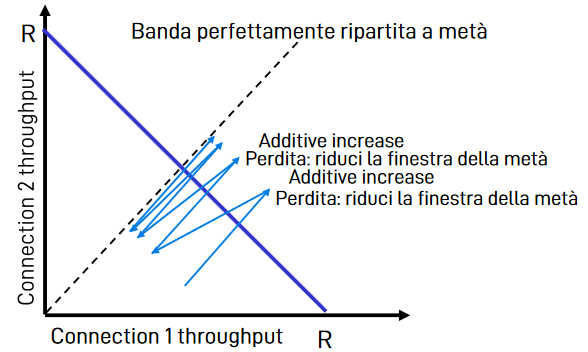
\includegraphics[width=0.5\textwidth]{03/congestione1.png}
                \caption{Grafico di congestione}
            \end{figure}
            Dal grafico si vede come nel tempo le connessioni oscillano verso il punto di intersezione, questo è dovuto al fatto che entrambe le connessioni aumentano la loro banda fino a che non si satura il link, a quel punto entrambe rilevano una perdita e riducono la loro banda dello stesso fattore, questo porta ad un \textit{fairness} tra le due connessioni.
    \subsection{Meccanismi per il controllo di congestione}
        Il controllo di congestione gestisce l'adattamento della cosiddetta finestra di congestione (\Acrshort*{CWND}$=$ numero di byte che il mittente può inviare). \newline
        In \Acrshort*{TCP} ci sono diversi algoritmi per il controllo di congestione, tra i più famosi ci sono: \begin{itemize}
            \item \textbf{In assenza di perdite}
                \subitem \Acrlong*{SS}
                \subitem \Acrlong*{CA}
            \item Per migliorare l'efficienza di \Acrshort*{TCP} in caso si verifichino perdite
                \subitem \Acrlong*{FRet}
                \subitem \Acrlong*{FRec}
        \end{itemize}
        \textbf{In ogni caso}: $\Acrshort*{W_T} = \min(\Acrshort*{CWND}, \Acrshort*{RWND}) = \min(\Acrshort*{CWND}, \Acrshort*{W_R}) $.
        \subsubsection{Slow Start}
            Il \Acrlong*{SS} è un algoritmo che prevede che per ogni \Acrshort*{ACK} ricevuto aumento di 1 \Acrshort*{MSS} la finestra di congestione, in questo modo la finestra aumenta esponenzialmente. Questo algoritmo è utilizzato quando la connessione è appena stata aperta e non si conosce la banda disponibile. Lo \Acrlong*{SS} termina quando la finestra di congestione raggiunge una soglia detta \acrfull*{SSThresh} e si passa al \textit{Congestion Avoidance}.
            \paragraph{Algoritmo della fase \Acrlong*{SS}}
            \begin{enumerate}
                \item \textbf{Inizializzazione} \begin{itemize}
                    \item \Acrshort*{CWND} = 1 \Acrshort*{MSS}
                    \item \Acrshort*{SSThresh} = \Acrshort*{RWND} (o \Acrshort*{RWND}/2)
                \end{itemize}
                \item \textbf{\Acrshort*{ACK} valido ricevuto}:\begin{itemize}
                    \item \Acrshort*{CWND} = \Acrshort*{CWND} + 1 \Acrshort*{MSS}
                    \item Sposto \Acrshort*{W_LOW} al primo segmento non \texttt{ACK'ato}
                    \item Se \Acrshort*{CWND} $ \geq $ \Acrshort*{SSThresh} allora passo alla fase di \textit{Congestion Avoidance}
                    \item Trasmetto nuovi segmenti (compresi tra \Acrshort*{W_LOW} e \Acrshort*{W_HIGH})
                \end{itemize}
                \item \textbf{Se scatta un \textit{timeout}}: \begin{itemize}
                    \item Abbasso \Acrshort*{SSThresh} a $\max(\Acrshort*{CWND}/2, 2)$
                    \item Aumento \Acrshort*{RTO} = $2\cdot \Acrshort*{RTO}$
                    \item Reimposto \Acrshort*{CWND} = 1 \Acrshort*{MSS}
                    \item Ritrasmetto il segmento in \textit{timeout} 
                \end{itemize}
            \end{enumerate}
            \subsubsection{\Acrlong*{CA}}
            Il \Acrlong*{CA} è un algoritmo che prevede che per ogni \Acrshort*{ACK} ricevuto aumento di $ \Acrshort*{MSS}\cdot \frac{\Acrshort*{MSS}}{\Acrshort*{CWND}} $ la finestra di congestione, in questo modo la finestra aumenta linearmente quando ``Trasmetto tutti i pacchetti della finestra attuale con successo''.
            Quindi per ogni \Acrshort*{RTT} in cui ricevo tutti gli \Acrshort*{ACK} attesi allora aumento di un segmento. Questo algoritmo segue un comportamento lineare e non esponenziale il che lo rende ideale per mantenere la rete stabile.
            \paragraph{Algoritmo della fase \Acrlong*{CA}}
            \begin{itemize}
                \item \textbf{Se ricevo un \Acrshort*{ACK} valido}:\begin{itemize}
                        \item \Acrshort*{CWND} = \Acrshort*{CWND} + $ \frac{\Acrshort*{MSS}}{\Acrshort*{CWND}} $ (in \underline{\textbf{byte}}!)
                        \item Sposto \Acrshort*{W_LOW} al primo segmento non \texttt{ACK'ato}
                        \item Trasmetto nuovi segmenti (compresi tra \Acrshort*{W_LOW} e \Acrshort*{W_HIGH})
                    \end{itemize}
                \item \textbf{Se scatta un \textit{timeout}}: \begin{itemize}
                        \item Passo alla fase di \Acrlong*{SS}
                        \item Abbasso $ \Acrshort*{SSThresh} = \max(\Acrshort*{CWND}/2, 2) $
                        \item Aumento \Acrshort*{RTO} = 2 \Acrshort*{RTO}
                        \item Reimposto \Acrshort*{CWND} = 1 \Acrshort*{MSS}
                        \item Ritrasmetto il segmento in timeout
                \end{itemize}
            \end{itemize}
        \subsubsection{Parametri i quali possono essere modificati}
            \begin{itemize}
                \item \acrfull*{CWND} -  Dimensione della finestra di congestione.
                \item \acrfull*{SSThresh} - Soglia di \Acrlong*{SS}.
                \item \acrfull*{RTO} - Tempo di ritrasmissione.
                \item \textbf{$\Acrshort*{W_LOW}\ \&\ \Acrshort*{W_HIGH}$} - Puntatori alla finestra di trasmissione.
            \end{itemize}
        \subsubsection{\acrfull*{FRet}}
            Il \Acrlong*{FRet} è un algoritmo facente parte della fase di \Acrlong*{CA} che prescrive la seguente condizione: se il mittente riceve tre \Acrshort*{ACK} duplicati allora ritrasmette il segmento richiesto dal \Acrshort*{ACK} duplicato, inoltre il fatto che il mittente riceva tre \Acrshort*{ACK} duplicati indica che c'è una congestione sulla rete si passa dunque alla fase di \textit{Fast Recovery}. Inoltre prendo in considerazione il valore di \texttt{RECOVER}$=\Acrshort*{W_HIGH}$ per determinare quanti segmenti sono stati trasmessi nella rete, in questo modo posso capire, una volta ricevuto un \Acrshort*{ACK} differente, quando e se il processo di \textit{Fast Retransmit} è terminato con successo.
        \subsubsection{\acrfull*{FRec}}
            Quando ricevo il 3° \Acrshort*{ACK} duplicato entro in \Acrlong*{FRec}, in questa fase avvengono diversi passaggi per evitare di saturare la rete: \begin{itemize}
                \item \textbf{Al 3° \Acrshort*{ACK} duplicato}:\begin{itemize}
                    \item \Acrshort*{SSThresh} = \Acrshort*{CWND}/2
                    \item Supponendo di aver perso solo il segmento in questione: \Acrshort*{CWND} = \Acrshort*{SSThresh} + 3 \Acrshort*{MSS}
                    \item Non sposto \Acrshort*{W_LOW}
                \end{itemize}
                \item \textbf{Se arrivano altri \Acrshort*{ACK} duplicati allora}: \begin{itemize}
                    \item \Acrshort*{CWND} = \Acrshort*{CWND} +1 \Acrshort*{MSS}
                    \item Non sposto \Acrshort*{W_LOW}
                \end{itemize}
                \item \textbf{Quando arriva un \Acrshort*{ACK} valido} (che comprende \texttt{RECOVER}): \begin{itemize}
                    \item \Acrshort*{CWND} = \Acrshort*{SSThresh}
                    \item Passo alla fase di \Acrlong*{CA}
                    \item Sposto \Acrshort*{W_LOW} al primo segmento non \texttt{ACK'ato}
                \end{itemize}
                \item \textbf{Se arriva un \Acrshort*{ACK} che \underline{non} comprende \texttt{RECOVER}}:\begin{itemize}
                    \item Ritrasmetto il primo segmento non \texttt{ACK'ato}
                    \item \Acrshort*{CWND} = \Acrshort*{CWND}-(numero di segmenti senza \Acrshort*{ACK})+1
                    \item Sposto \Acrshort*{W_LOW} al primo segmento non \texttt{ACK'ato}
                \end{itemize}
            \end{itemize}
            
            \begin{figure}[H]
                \centering
                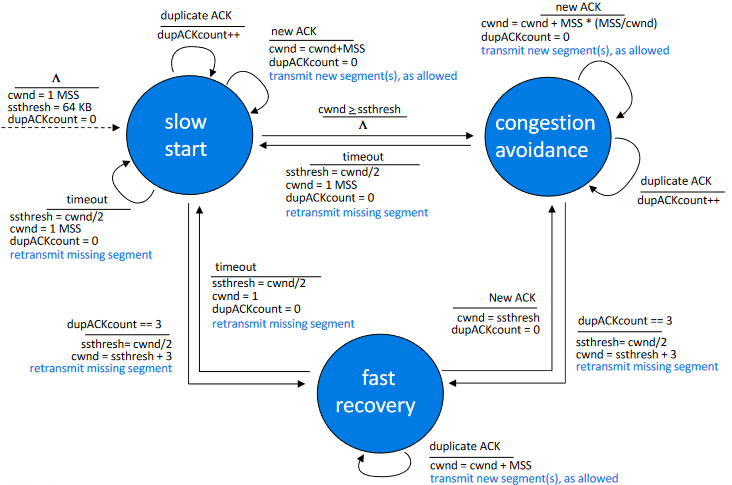
\includegraphics[width=0.6\textwidth]{03/macchinaStatiTCP.png}
                \caption{Macchina a stati di \Acrshort*{TCP}}
            \end{figure}
        \subsubsection{Problemi di equità (\textit{fairness}) in \Acrshort*{TCP}}
            In quanto le applicazione multimediali usano di rado \Acrshort*{TCP} per la trasmissione (ma usano \Acrshort*{UDP}), queste non sono soggette ai controlli di congestione, quindi le connessioni \Acrshort*{TCP} sono penalizzate. Questo avviene in quanto le connessioni \Acrshort*{UDP} trasmettono a velocità costante indipendentemente da fattori esterni.\newline
            Se invece abbiamo due \textit{host} che usano \Acrshort*{TCP} e uno apre (ad es.) $ 9 $ connessioni mentre l'altro ne apre $ 1 $ allora il primo avrà un \textit{throughput} di $ \frac{R}2 $ mentre il secondo avrà un \textit{throughput} di $ \frac{R} {10} $.
    \subsection{Altri algoritmi più recenti per il controllo di congestione}
        Negli algoritmi visti fino ad ora il processo di "rallentamento" della trasmissione avveniva solo in caso di perdita di pacchetti, questo però permette di regolare la banda solo quando è troppo tardi, in quanto deve avvenire una perdita prima che il mittente si renda conto che c'è una congestione. Per ovviare a questo problema sono stati introdotti nuovi algoritmi che permettono di regolare la banda. Questi algoritmi sono: \begin{itemize}
            \item \acrfull*{CUBIC}
            \item \acrfull*{BBR}
            \item \acrfull*{QUIC}
        \end{itemize}
        \subsubsection{\acrfull*{CUBIC}}
            L'algoritmo \Acrshort*{CUBIC} fa variare la lunghezza della finestra di congestione secondo una funzione cubica nel tempo, questo ne migliora la scalabilità e la stabilità. Questo algoritmo è stato introdotto nel kernel di \texttt{Linux} a partire dalla versione 2.6.19, mentre in \texttt{Windows} è stato introdotto a partire dal 2017.
            \paragraph{Principi del funzionamento} Per un migliore utilizzo e stabilità della rete \Acrshort*{CUBIC} usa sia sia la parte concava che quella convessa della funzione cubica per regolare la finestra di congestione. 
            $$
                \Acrshort*{CWND}_{cubic}(t) = C(t-K)^3 + \Acrshort*{CWND}_{max}
            $$
            Dove $ C $ è una costante, $ K = \sqrt[3]{\frac{\Acrshort*{CWND}_{max}(1-\beta)}{C}} $ e $ \Acrshort*{CWND}_{max} $ è la dimensione massima della finestra di congestione. Per lo standard \texttt{\Acrshort*{RFC} 8312} $ C = 0.4 $ e $ \beta = 0.7 $, ma dopo che è stata rilevata una congestione allora $ \beta = 0.5 $. Inoltre questo algoritmo è "\Acrshort*{TCP}\textit{-friendly}" ovvero non penalizza i flussi \Acrshort*{TCP} legacy che condividono la stessa rete.
        \subsubsection{\acrfull*{BBR}}
            L'algoritmo \Acrshort*{BBR} è un algoritmo di controllo di congestione che cerca di massimizzare il \textit{throughput} e minimizzare il ritardo. Questo algoritmo è stato introdotto da \texttt{Google} nel 2016 e si basa non sul rilevamento di perdite ma su due parametri: \begin{itemize}
                \item \textbf{Bottleneck Bandwidth} La banda disponibile sul \textit{bottleneck}.
                \item \textbf{Round-trip propagation time} Il tempo di propagazione del pacchetto.
            \end{itemize}
            Il funzionamento a grandi linee prevede la trasmissione di pacchetti ad una velocità che non \textit{dovrebbe} saturare la rete. Questo infatti è progettato per ridurre la finestra di congestione prima che si verifichi una perdita, in questo modo si dovrebbe riuscire a limitare ritrasmissioni inutili. Un vantaggio di \Acrshort*{BBR} è quello che solo il \textit{server} lo deve implementare e non anche il \textit{client}. Il concetto usato è quello di \textit{pacing} ovvero inserisco nuovi pacchetti nella \Acrshort*{CWND} solo quando il nodo più lento della rete è pronto a riceverli.
            \paragraph{Migliore produttività} Secondo \textit{Google} \Acrshort*{BBR} con un \textit{link} a $10$ Gbps che invia dati lungo un percorso con \Acrshort*{RTT} di $100$ms con tasso di perdita dell'$1\%$ riesce a raggiungere un \textit{throughput} di $3,3$Mbit/s con \Acrshort*{CUBIC} e di $9100$Mbit/s con \texttt{BBR}. Questo è ideale nel caso di connessioni \texttt{\Acrshort*{HTTP}/2} che sfruttano una singola connessione per trasmettere dati.
            \paragraph{Latenza inferiore} \Acrshort*{BBR} riesce a mantenere una latenza inferiore rispetto a \Acrshort*{CUBIC} in quanto riesce a mantenere la banda costante e non satura la rete. Vari studi (sempre di \textit{Google}) hanno dimostrato che su un collegamento di $10$ Mbps con \Acrshort*{RTT} di $40$ ms ed un \textit{bottleneck} di $1000$ pacchetti la latenza di \Acrshort*{BBR} è di soli $43$ ms contro i $1090$ ms di \Acrshort*{CUBIC}.
        \subsubsection{\acrfull*{QUIC}}
            \Acrshort*{QUIC} è un protocollo di trasporto sviluppato da \texttt{Google} nel 2012 e si prefissa il raggiungimento di due obbiettivi:\begin{itemize}
                \item Evitare fenomeni di \textit{head-of-line blocking}
                \item Ridurre la latenza di \Acrshort*{TCP}
            \end{itemize}
            \Acrshort*{QUIC} può essere implementato a livello applicazione, oltre che a livello di \textit{kernel}. Lo \textit{use case} di questo dovrebbe essere quello delle connessioni \texttt{\Acrshort*{HTTP}/3}. Il principio di funzionamento di questo è che i pacchetti vengono trasmessi tramite una connessione \Acrshort*{UDP} e non \Acrshort*{TCP}, questo permette di evitare i problemi di \textit{head-of-line blocking} in quanto se un pacchetto viene perso allora non si bloccano tutti i pacchetti successivi. Inoltre \Acrshort*{QUIC} permette di ridurre l'\textit{overhead} di connessione in quando incorpora in se stesso lo scambio delle chiavi (o \textit{handshake}) di \Acrshort*{TLS}.
    \subsection{Conclusioni}
        \subsubsection{Meglio dunque \Acrshort*{TCP} o \Acrshort*{UDP}?}
        La scelta tra \Acrshort*{TCP} e \Acrshort*{UDP} dipende da cosa si vuole fare, se si vuole trasmettere dati in modo affidabile e si vuole evitare di saturare la rete allora si deve usare \Acrshort*{TCP}, se invece si vuole trasmettere dati in modo veloce e non si vuole preoccuparsi di perdite di pacchetti allora si deve usare \Acrshort*{UDP}. Questa scelta però non è così libera come sembra, in quanto se si vuole usare il protocollo \Acrshort*{QUIC} necessitiamo di connessione \Acrshort*{UDP} ma molta della nostra infrastruttura blocca le connessioni di questo tipo in quanto non avviene un controllo di congestione e quindi si rischia di saturare la rete. Google ha provato a mostrare come \Acrshort*{QUIC} sia migliore di \Acrshort*{TCP} cercando di "sbloccare" la rete per questo tipo di connessioni, detto ciò i prodotti della serie \textit{chromium} aprono in contemporanea una connessione \Acrshort*{TCP} e una connessione \Acrshort*{UDP} e scelgono quella che ha il \textit{throughput} migliore. 
        \subsubsection{Cambio di rete}
            Con le connessioni \Acrshort*{TCP} le \textit{socket} vengono identificate dalla quadrupla: \texttt{(\Acrshort*{IP} M.,\Acrshort*{IP} D., Porta M., Porta D.)}, se si cambia rete allora si cambia anche l'indirizzo \Acrshort*{IP} e quindi la connessione \Acrshort*{TCP} viene persa. Con \Acrshort*{QUIC} invece la connessione viene mantenuta in quanto la \textit{socket} è identificata da un \texttt{ID} e non dall'indirizzo \Acrshort*{IP}.